%%%%%%%%%%%%%%%%%%%%%%%%%%%%%%%%%%%%%%%%%
% Beamer Presentation
% LaTeX Template
% Version 1.0 (10/11/12)
%
% This template has been downloaded from:
% http://www.LaTeXTemplates.com
%
% License:
% CC BY-NC-SA 3.0 (http://creativecommons.org/licenses/by-nc-sa/3.0/)
%
%%%%%%%%%%%%%%%%%%%%%%%%%%%%%%%%%%%%%%%%%

%----------------------------------------------------------------------------------------
%	PACKAGES AND THEMES
%----------------------------------------------------------------------------------------

\documentclass{beamer}

\mode<presentation> {

% The Beamer class comes with a number of default slide themes
% which change the colors and layouts of slides. Below this is a list
% of all the themes, uncomment each in turn to see what they look like.

%\usetheme{default}
%\usetheme{AnnArbor}
%\usetheme{Antibes}
%\usetheme{Bergen}
%\usetheme{Berkeley}
%\usetheme{Berlin}
%\usetheme{Boadilla}
%\usetheme{CambridgeUS}
%\usetheme{Copenhagen}
%\usetheme{Darmstadt}
%\usetheme{Dresden}
%\usetheme{Frankfurt}
%\usetheme{Goettingen}
%\usetheme{Hannover}
%\usetheme{Ilmenau}
%\usetheme{JuanLesPins}
%\usetheme{Luebeck}
\usetheme{Madrid}
%\usetheme{Malmoe}
%\usetheme{Marburg}
%\usetheme{Montpellier}
%\usetheme{PaloAlto}
%\usetheme{Pittsburgh}
%\usetheme{Rochester}
%\usetheme{Singapore}
%\usetheme{Szeged}
%\usetheme{Warsaw}

% As well as themes, the Beamer class has a number of color themes
% for any slide theme. Uncomment each of these in turn to see how it
% changes the colors of your current slide theme.

%\usecolortheme{albatross}
%\usecolortheme{beaver}
%\usecolortheme{beetle}
%\usecolortheme{crane}
%\usecolortheme{dolphin}
%\usecolortheme{dove}
%\usecolortheme{fly}
%\usecolortheme{lily}
%\usecolortheme{orchid}
%\usecolortheme{rose}
%\usecolortheme{seagull}
%\usecolortheme{seahorse}
%\usecolortheme{whale}
%\usecolortheme{wolverine}

%\setbeamertemplate{footline} % To remove the footer line in all slides uncomment this line
%\setbeamertemplate{footline}[page number] % To replace the footer line in all slides with a simple slide count uncomment this line

%\setbeamertemplate{navigation symbols}{} % To remove the navigation symbols from the bottom of all slides uncomment this line
}

\usepackage{graphicx} % Allows including images
\usepackage{booktabs} % Allows the use of \toprule, \midrule and \bottomrule in tables

%----------------------------------------------------------------------------------------
%	TITLE PAGE
%----------------------------------------------------------------------------------------

\title[State Estimation]{State Estimation of Induction Machine using UKF} % The short title appears at the bottom of every slide, the full title is only on the title page

\author{Ram Milan Verma} % Your name
\institute[IITB] % Your institution as it will appear on the bottom of every slide, may be shorthand to save space
{
Indian Institute of Technology, Bombay \\ % Your institution for the title page
\medskip
\textbf{Course Project - CL 653} % Your email address
}
\date{\today} % Date, can be changed to a custom date

\begin{document}

\begin{frame}
\titlepage % Print the title page as the first slide
\end{frame}

\begin{frame}
\frametitle{Contents} % Table of contents slide, comment this block out to remove it
\tableofcontents % Throughout your presentation, if you choose to use \section{} and \subsection{} commands, these will automatically be printed on this slide as an overview of your presentation
\end{frame}

%----------------------------------------------------------------------------------------
%	PRESENTATION SLIDES
%----------------------------------------------------------------------------------------

%------------------------------------------------
\section{Importance/Idea of UKF} % Sections can be created in order to organize your presentation into discrete blocks, all sections and subsections are automatically printed in the table of contents as an overview of the talk
%------------------------------------------------

%\subsection{Subsection Example} % A subsection can be created just before a set of slides with a common theme to further break down your presentation into chunks

\begin{frame}
\frametitle{Importance of UKF(Unscented Kalman Filter)}
\begin{itemize}
    \item Derivative free sampling based filter.
    \item Uses deterministic sampling and associates weights.
    \item Numerical approximations of first and second moments can be found using sample points chosen.
    \item Sample point generation is called \textbf{sigma point generation}.
    \item Sigma point is generated symmetrically around the mean.
    \item Hence, works well for signals with \textbf{unimodal and symmetric} probability densities.
\end{itemize}
\end{frame}

%------------------------------------------------
\section{Details of algorithm of UKF}
\begin{frame}
\frametitle{Unscented Kalman Filter}
\begin{block}{Augmented Quantities}
\begin{enumerate}
    \item $\chi(k-1)=[\textbf{X}(k-1)^T, \textbf{d}(k-1)^T, \textbf{v}(k-1)^T]^T$
    \item It's mean, $\widehat{\chi}(k-1|k-1)=[\widehat{X}(k-1|k-1)^T, \overline{0}^T, \space \overline{0}^T ]^T$\\
    \item Covariance matrix,$\textbf{P}^a(k-1|k-1) = diag[\textbf{P}(k-1|k-1),  \textbf{Q},  \textbf{R}]$
\end{enumerate}


\end{block}

\begin{block}{Sigma Point generation}
\begin{itemize}
    \item \textbf{M}=dim(\textbf{$\chi$});\space \ Number of samples, $N_{s}=2M+1$
    \item $\chi^{(1)}(k-1|k-1)=\widehat{\chi}(k-1|k-1)$
    \item $\chi^{(i+1)}(k-1|k-1)=\widehat{\chi}(k-1|k-1) + \rho \sqrt{P^a(k-1|k-1)}\zeta^{(i)}$
    \item $\chi^{(i+M+1)}(k-1|k-1)=\widehat{\chi}(k-1|k-1) - \rho \sqrt{P^a(k-1|k-1)}\zeta^{(i)}$\\
    where $\zeta^{(i)}=[0,0,...,1,0,0]^T$ \ i=1,...,M;\ $\rho=\sqrt{M+\kappa}$\\
    $\kappa\ $(tuning parameter)$\ =1\ or\ (3-M) \ $(A Typical choice)
\end{itemize}
\end{block}

\end{frame}

%------------------------------------------------

\begin{frame}
\frametitle{Unscented Kalman Filter}
\begin{block}{Weights}
\begin{itemize}
    \item Weights are chosen such that $\sum \omega_{i}=1$ and weighted sample average equals $\widehat{\chi}(k-1|k-1)$
    \item $\omega_1=\frac{\kappa}{M+\kappa}$
    \item $\omega_{i+1}=\omega_{i+M+1}=\frac{1}{2(M+\kappa)}$ \ \ \ For i=1,..,M
\end{itemize}
\end{block}
\begin{block}{Propagation using system and measurement models}
\begin{itemize}
    \item state propagation
        \begin{itemize}
            \item Integrate the model equation for each sample points.
            \item Get the weighted sum as sample mean, $\widehat{X}(k|k-1)=\sum\omega_i\widehat{X}^{(i)}(k|k-1)$
        \end{itemize}
    \item Measurement prediction
        \begin{itemize}
            \item Get $Y^{(i)}(k|k-1)$ by substituting $\widehat{X}^{(i)}(k|k-1)$ 
            \item $\widehat{Y}(k|k-1)=\sum\omega_i\widehat{Y}^{(i)}(k|k-1)$
        \end{itemize}
\end{itemize}
\end{block}
\end{frame}

%------------------------------------------------
\begin{frame}{Unscented Kalman Filter}
\begin{block}{Defining error and covariances}
\begin{itemize}
    \item $\varepsilon^{(i)}(k|k-1) = \widehat{X}^{(i)}(k|k-1) - \widehat{X}(k|k-1)$
    \item $\epsilon^{(i)}(k)= \widehat{Y}^{(i)}(k|k-1) - \widehat{Y}(k|k-1)$
    \item Covariances
        \begin{itemize}
            \item $P_{\varepsilon\varepsilon}(k|k-1)\approx \sum\omega_i\varepsilon^{(i)}(k|k-1)[\varepsilon^{(i)}(k|k-1)]^T$
            \item $P_{\varepsilon\epsilon}(k)\approx \sum\omega_i\varepsilon^{(i)}(k|k-1)[\epsilon^{(i)}(k)]^T$
            \item $P_{\epsilon\epsilon}(k)\approx \sum\omega_i\epsilon^{(i)}(k)[\epsilon^{(i)}(k)]^T$
        \end{itemize}
\end{itemize}
\end{block}
\begin{block}{Kalman Update}
\begin{itemize}
    \item $L(k)=P_{\varepsilon\epsilon}(k)\ P_{\epsilon\epsilon}(k)^{-1}$
    \item innovation, $e(k) =Y(k) - \widehat{Y}(k|k-1)$
    \item $\widehat{X}(k|k)=\widehat{X}(k|k-1)+ L(k) \ e(k)$
    \item $P(k|k)= P_{\varepsilon\varepsilon}(k|k-1) - L(k)P_{\epsilon\epsilon}(k)L(k)^T$
\end{itemize}
\end{block}
\end{frame}
%------------------------------------------------
\section{Model equations and Parameters}
\begin{frame}{Model equations}
\begin{itemize}
    \item State space model of system
    \begin{equation}
        \frac{dx_1}{dt}=k_1x_1 + z_1x_2+k_2x_3+z_2
    \end{equation}
    \begin{equation}
        \frac{dx_2}{dt}=z_1x_1 +k_1x_2+k_2x_4
    \end{equation}
    \begin{equation}
        \frac{dx_3}{dt}=k_3x_1+k_4x_3+(z_1-x_5)x_4
    \end{equation}
    \begin{equation}
        \frac{dx_4}{dt}=k_3x_2-(z_1-x_5)x_3+k_4x_4
    \end{equation}
    \begin{equation}
        \frac{dx_5}{dt}=k_5(x_1x_4-x_2x_3)+k_6z_3
    \end{equation}
    where $x_1,x_2 \ and \ x_3,x_4$ are components of stator and rotor flux; $x_5$ is angular velocity; $z_1,z_2,z_3$ are inputs indicating frequency, amplitude and load torque
\end{itemize} 
\end{frame}
%------------------------------------------------
\begin{frame}{Measurement model and Parameters}
\begin{itemize}
    \item Measurement model equations
    \begin{equation}
        y_1=k_7x_1+k8x_3
    \end{equation}
    \begin{equation}
        y2=k_7x_2+k_8x_4
    \end{equation}
    \item x(0)=$[0.2,-0.6,-0.4,0.1,0.3]^T\ ;\ Q=10^{-4}I_{5x5};$\\
    $\ R=10^{-2}I_{2x2}\ ; T_s\ =0.1\ sec; \ P(0|0)=I_{5x5};\ N=500$
    \begin{table}[h!]
    \tiny
  \begin{center}
    \caption{Parameters and inputs}
    \label{tab:table1}
    \begin{tabular}{r|r|r|r|r|r|r|r|r|r|l} % <-- Alignments: 1st column left, 2nd middle and 3rd right, with vertical lines in between
      $k1$ & $k_2$ & $k_3$ & $k_4$ & $k_5$ & $k_6$ & $k_7$ & $k_8$ &$z_1$ & $z_2$ & $z_3$ \\
      \hline
      -0.186 & 0.178 & 0.225 & -0.234 & -0.081&4.643& -4.448 & 1& 1&1 & 0
    \end{tabular}
  \end{center}
\end{table}
    
    
\end{itemize}
    
\end{frame}
%------------------------------------------------
\section{Linearisation Point for KF}
\begin{frame}{Linearisation point for KF}
\begin{itemize}
    \item Used \textbf{fsolve} function of MATLAB.
    \item it takes initial point $(x_0)$ as one argument to perform search.
    \item Used \textbf{feval} to check the correctness of steady state point obtained.
    \item For $x_0$=[0 0 0 1 1] or [0 -1 0.5 -1 1]
    \item $x_{ss}=[0.0148\ -0.9998\ 0.0143\  -0.9613\  1.0000]$
    \item Output of feval: \ \ 1.0e-08 *[0.0000    0.0000    0.0481   -0.1631   -0.0023]
\end{itemize}
    
\end{frame}
%-------------------------Results section--------------------------------
\section{Results}
%------------------------------------------------TRUE VS ESTIMATED--------------
\begin{frame}
\frametitle{Results: True Vs Estimated(All Filter)}
\begin{figure}
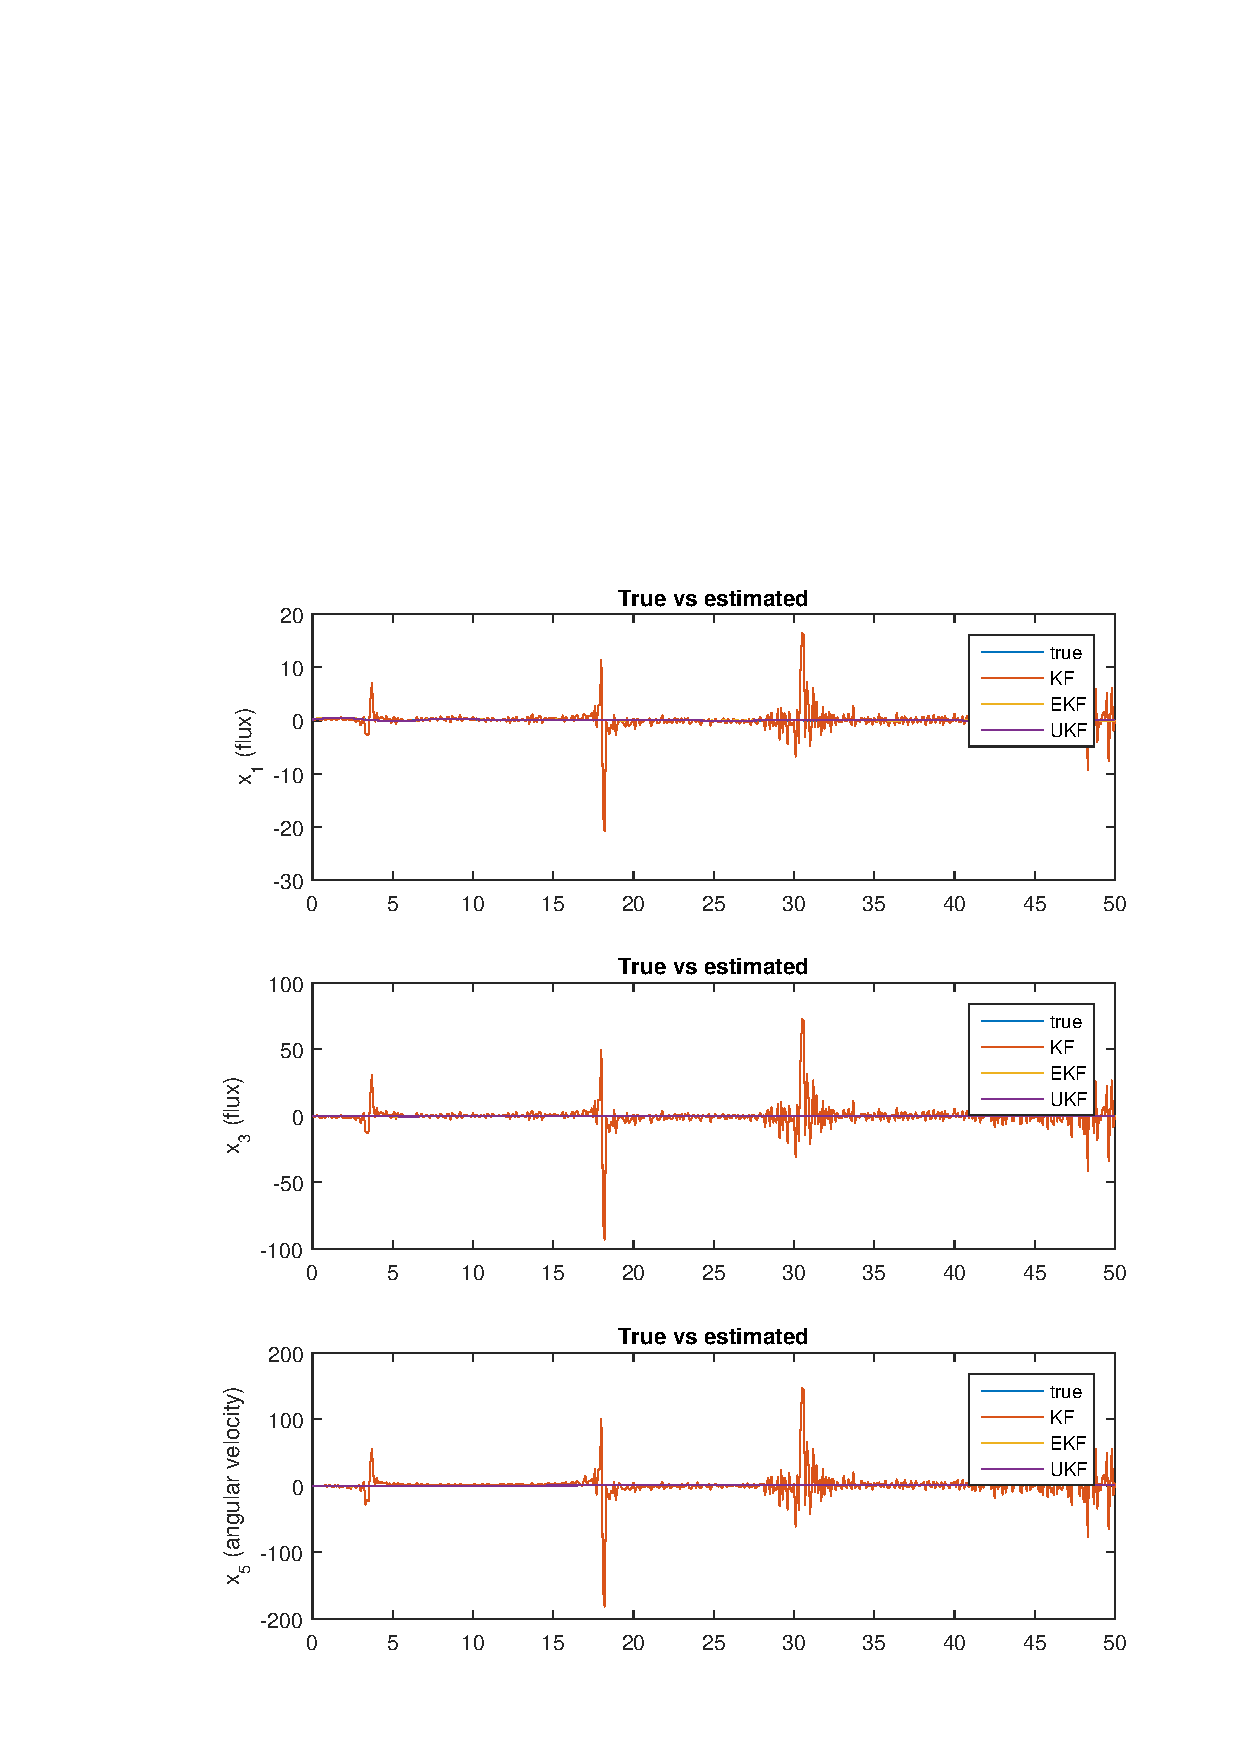
\includegraphics[width=0.8\linewidth]{plots/true_vs_estimated_all.png}
\end{figure}
\end{frame}
%------------------------------------------------
\begin{frame}
\frametitle{Results:True Vs Estimated(EKF and UKF)}

\begin{figure}
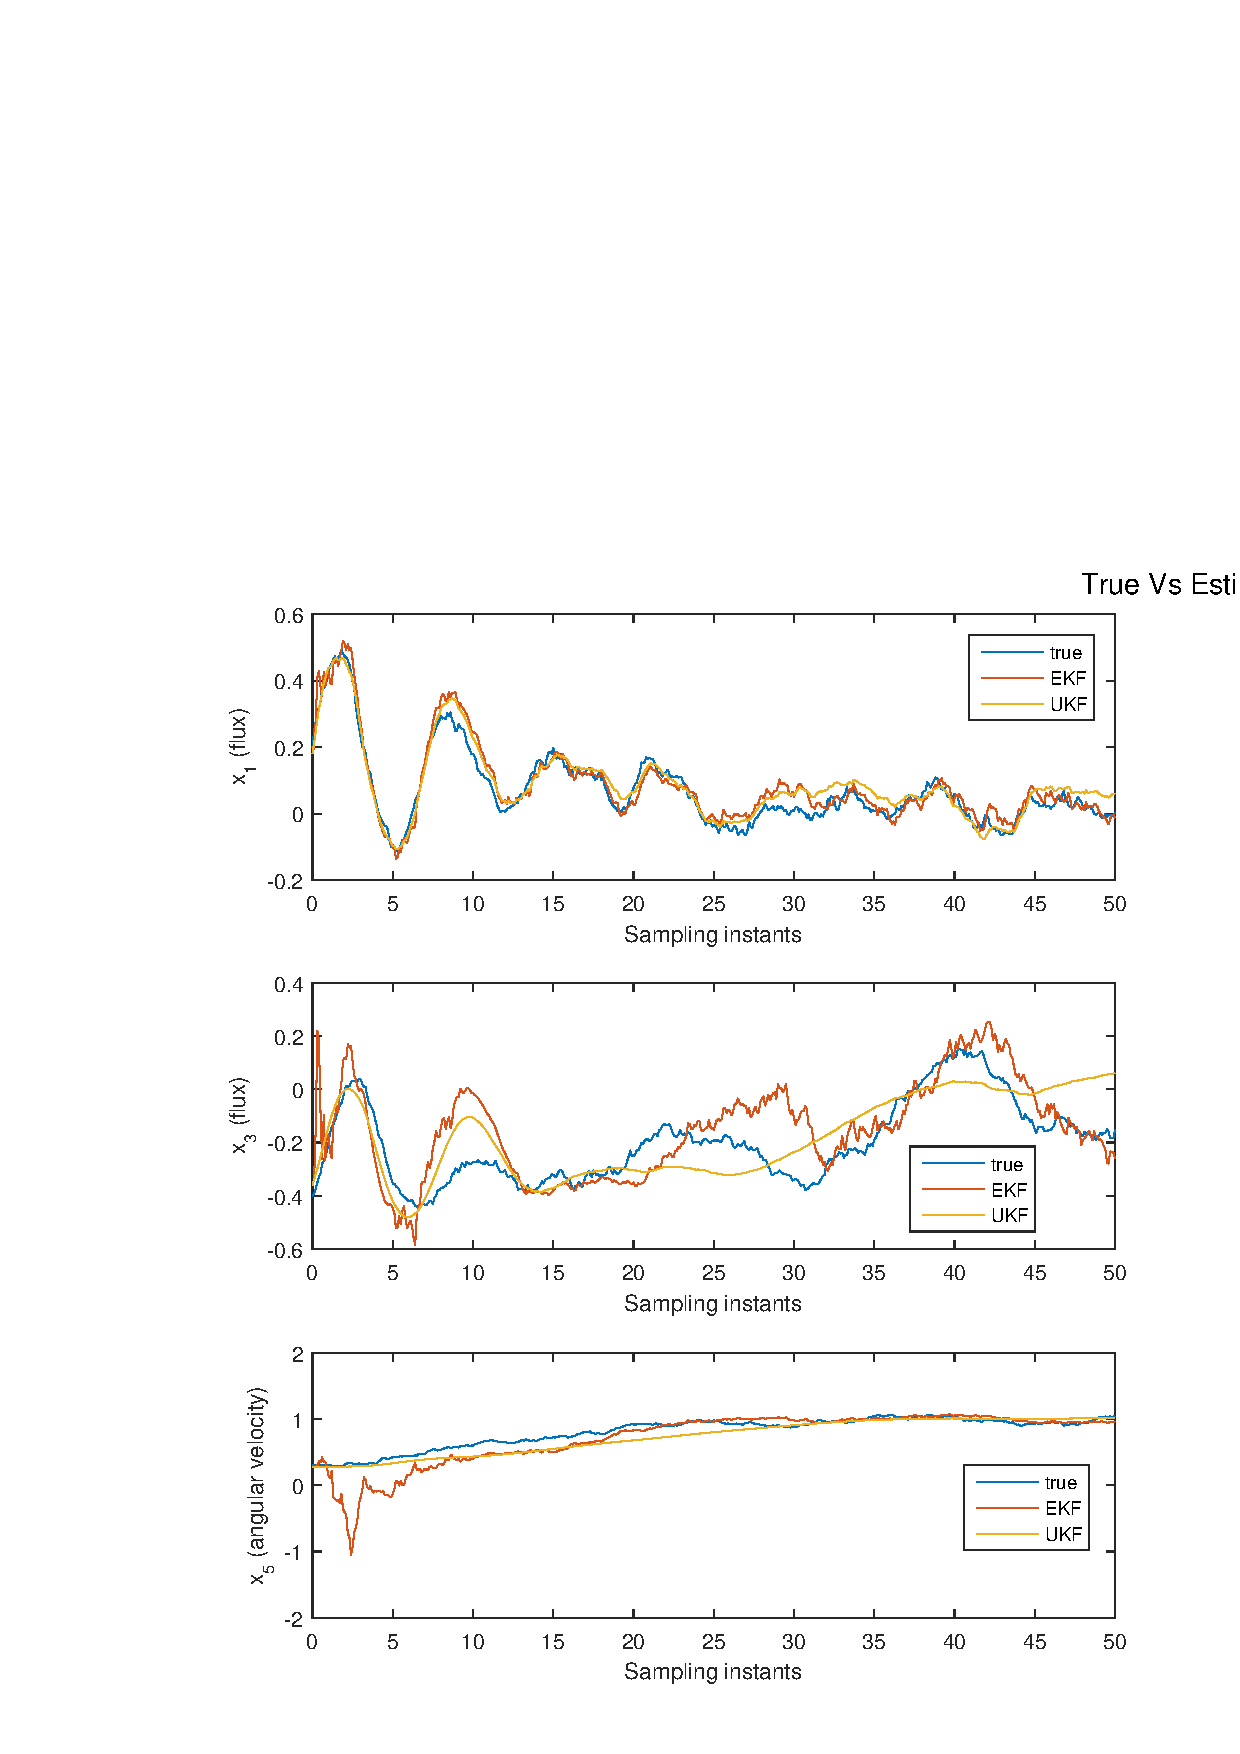
\includegraphics[width=0.8\linewidth]{plots/true_vs_estimated_noKF.png}
\end{figure}
\end{frame}
%------------------------------------------------INNOVATION---------------------
\begin{frame}
\frametitle{Results: Innovation(All Filter)}

\begin{figure}
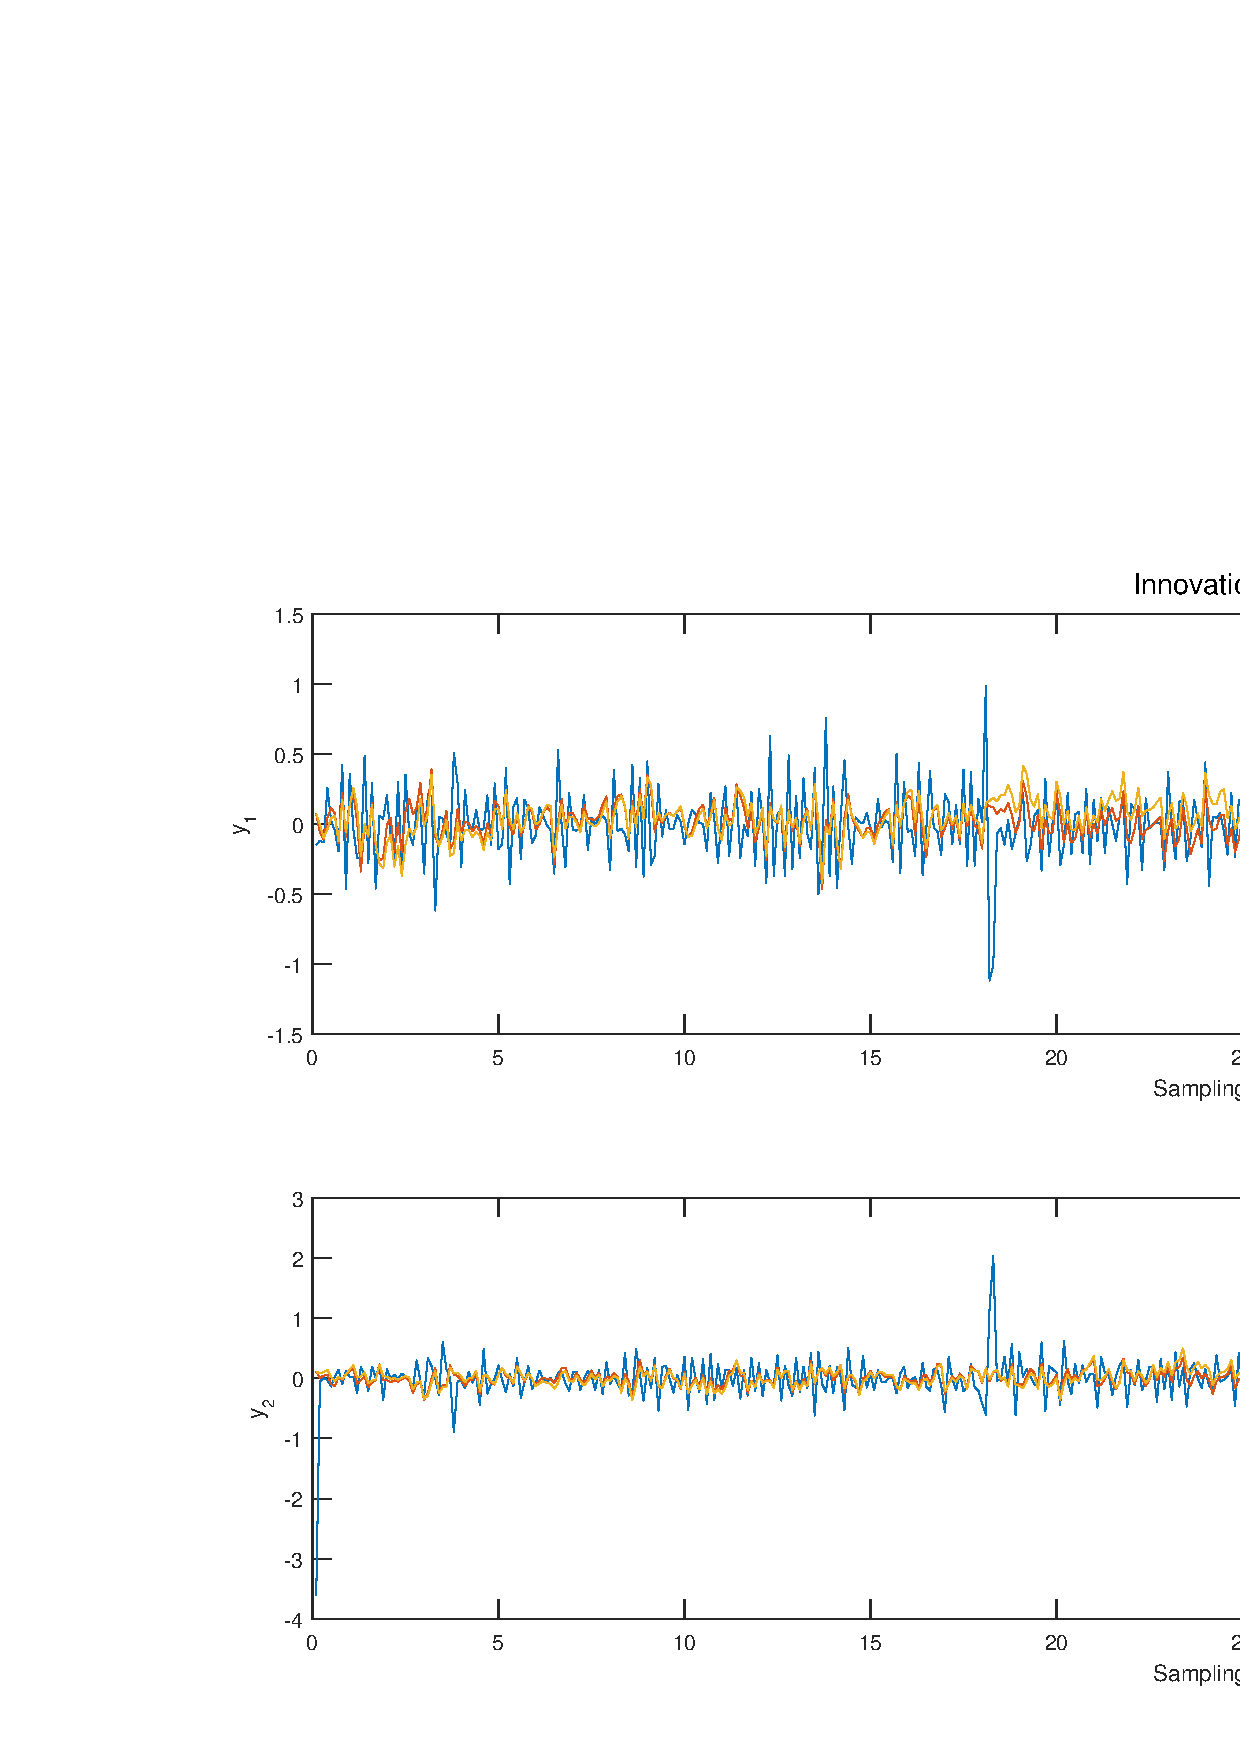
\includegraphics[width=0.8\linewidth]{plots/innovation_all.png}
\end{figure}
\end{frame}
%------------------------------------------------
\begin{frame}
\frametitle{Results: Innovation(EKF and UKF)}

\begin{figure}
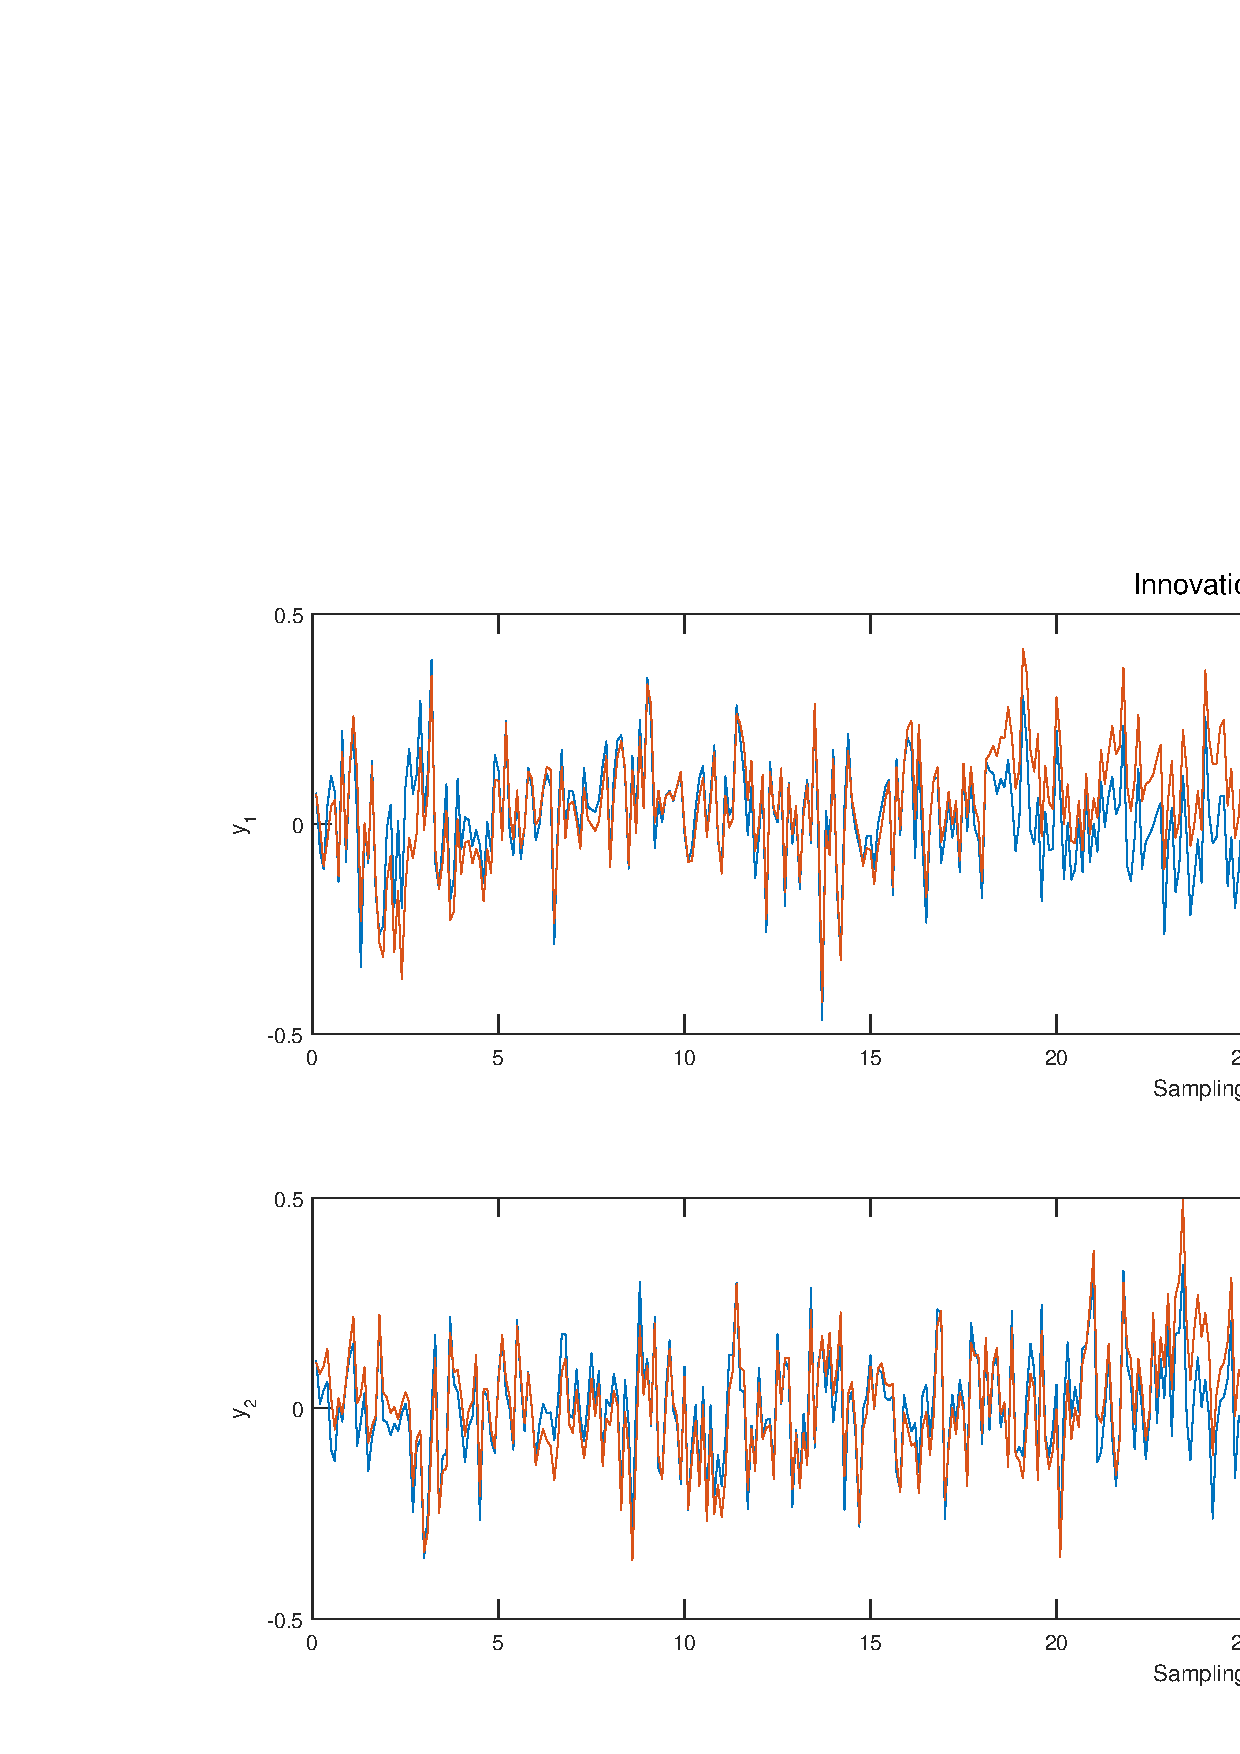
\includegraphics[width=0.8\linewidth]{plots/innovation_noKF.png}
\end{figure}
\end{frame}
%-----------------------------------------------SPECTRAL RADII----------------
\begin{frame}
\frametitle{Results: Spectral Radii(All on same plot)}
\begin{figure}
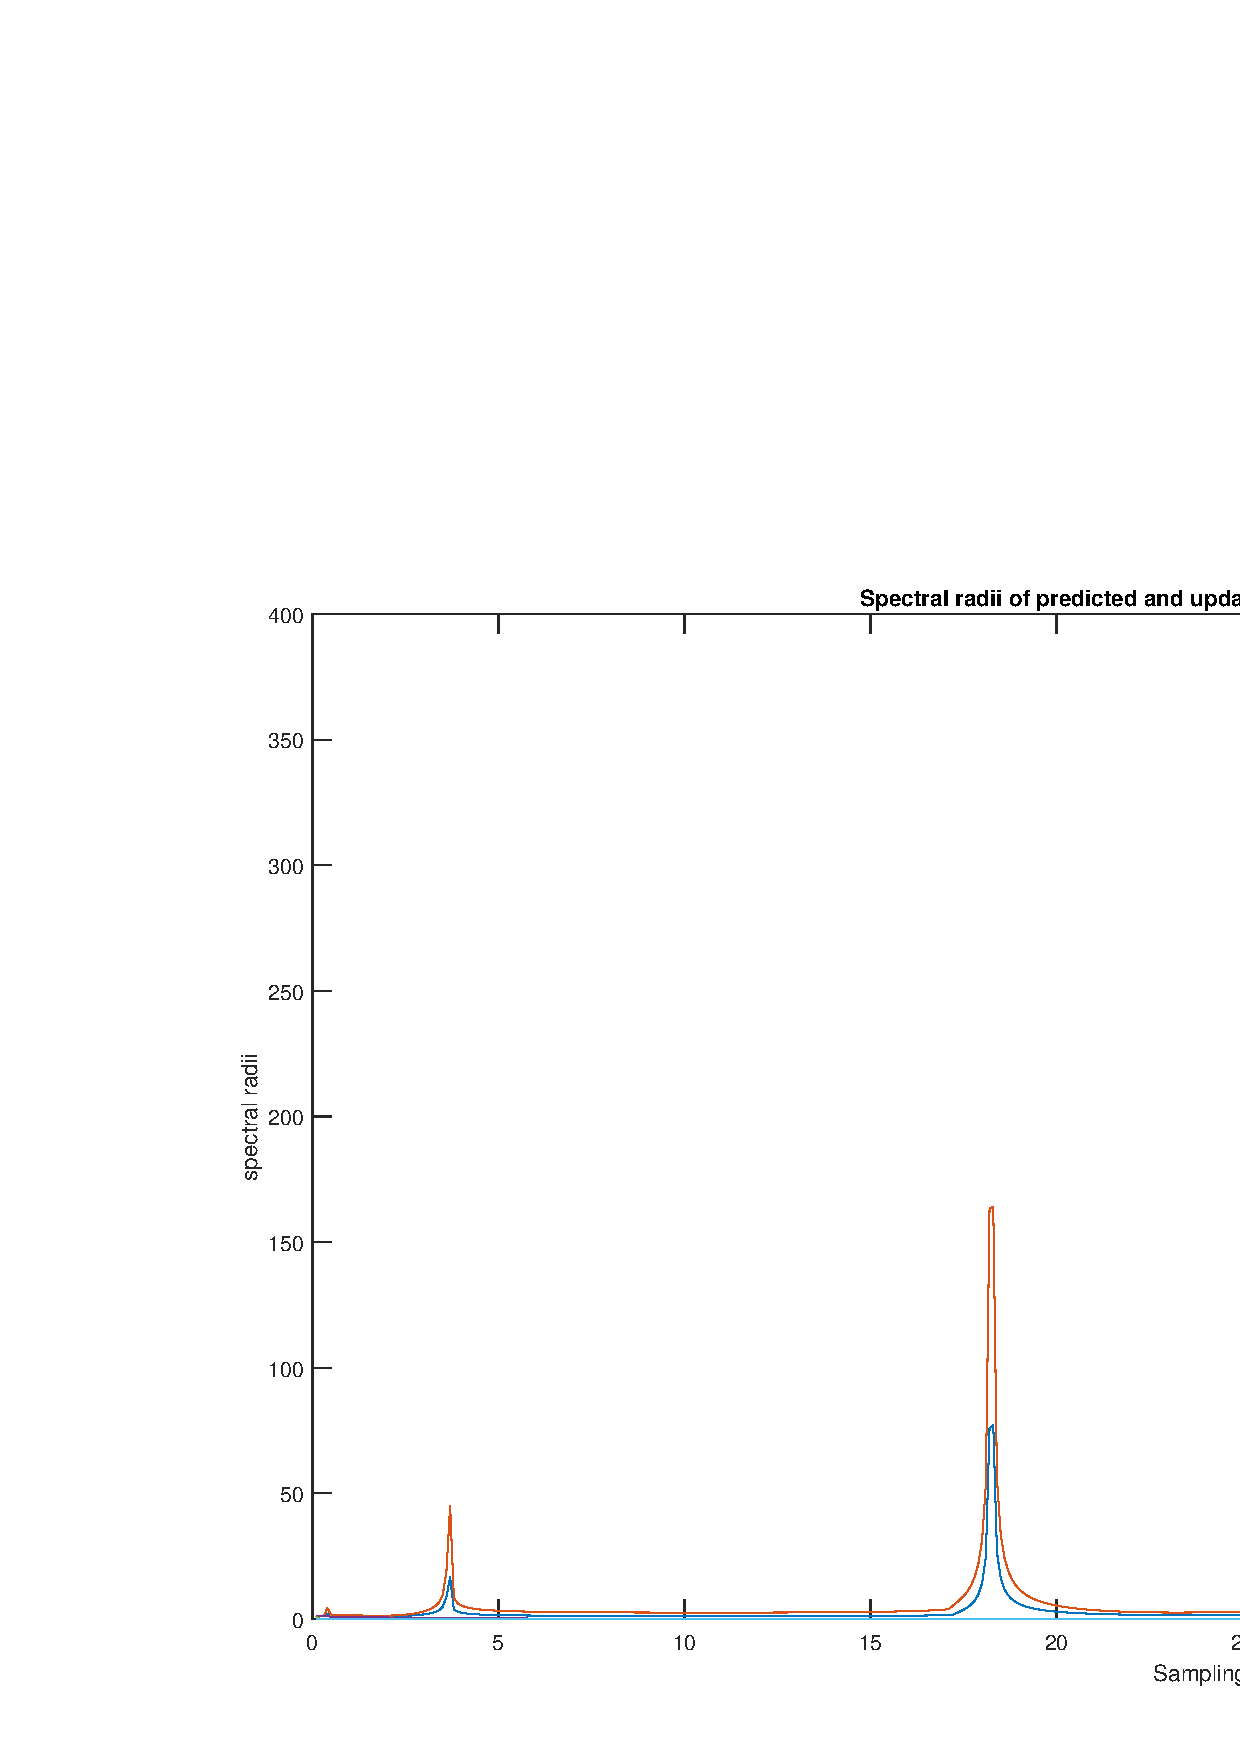
\includegraphics[width=0.8\linewidth]{plots/spectral_radii_all.png}
\end{figure}
\end{frame}
%------------------------------------------------
\begin{frame}
\frametitle{Results: Spectral Radii(subplots)}
\begin{figure}
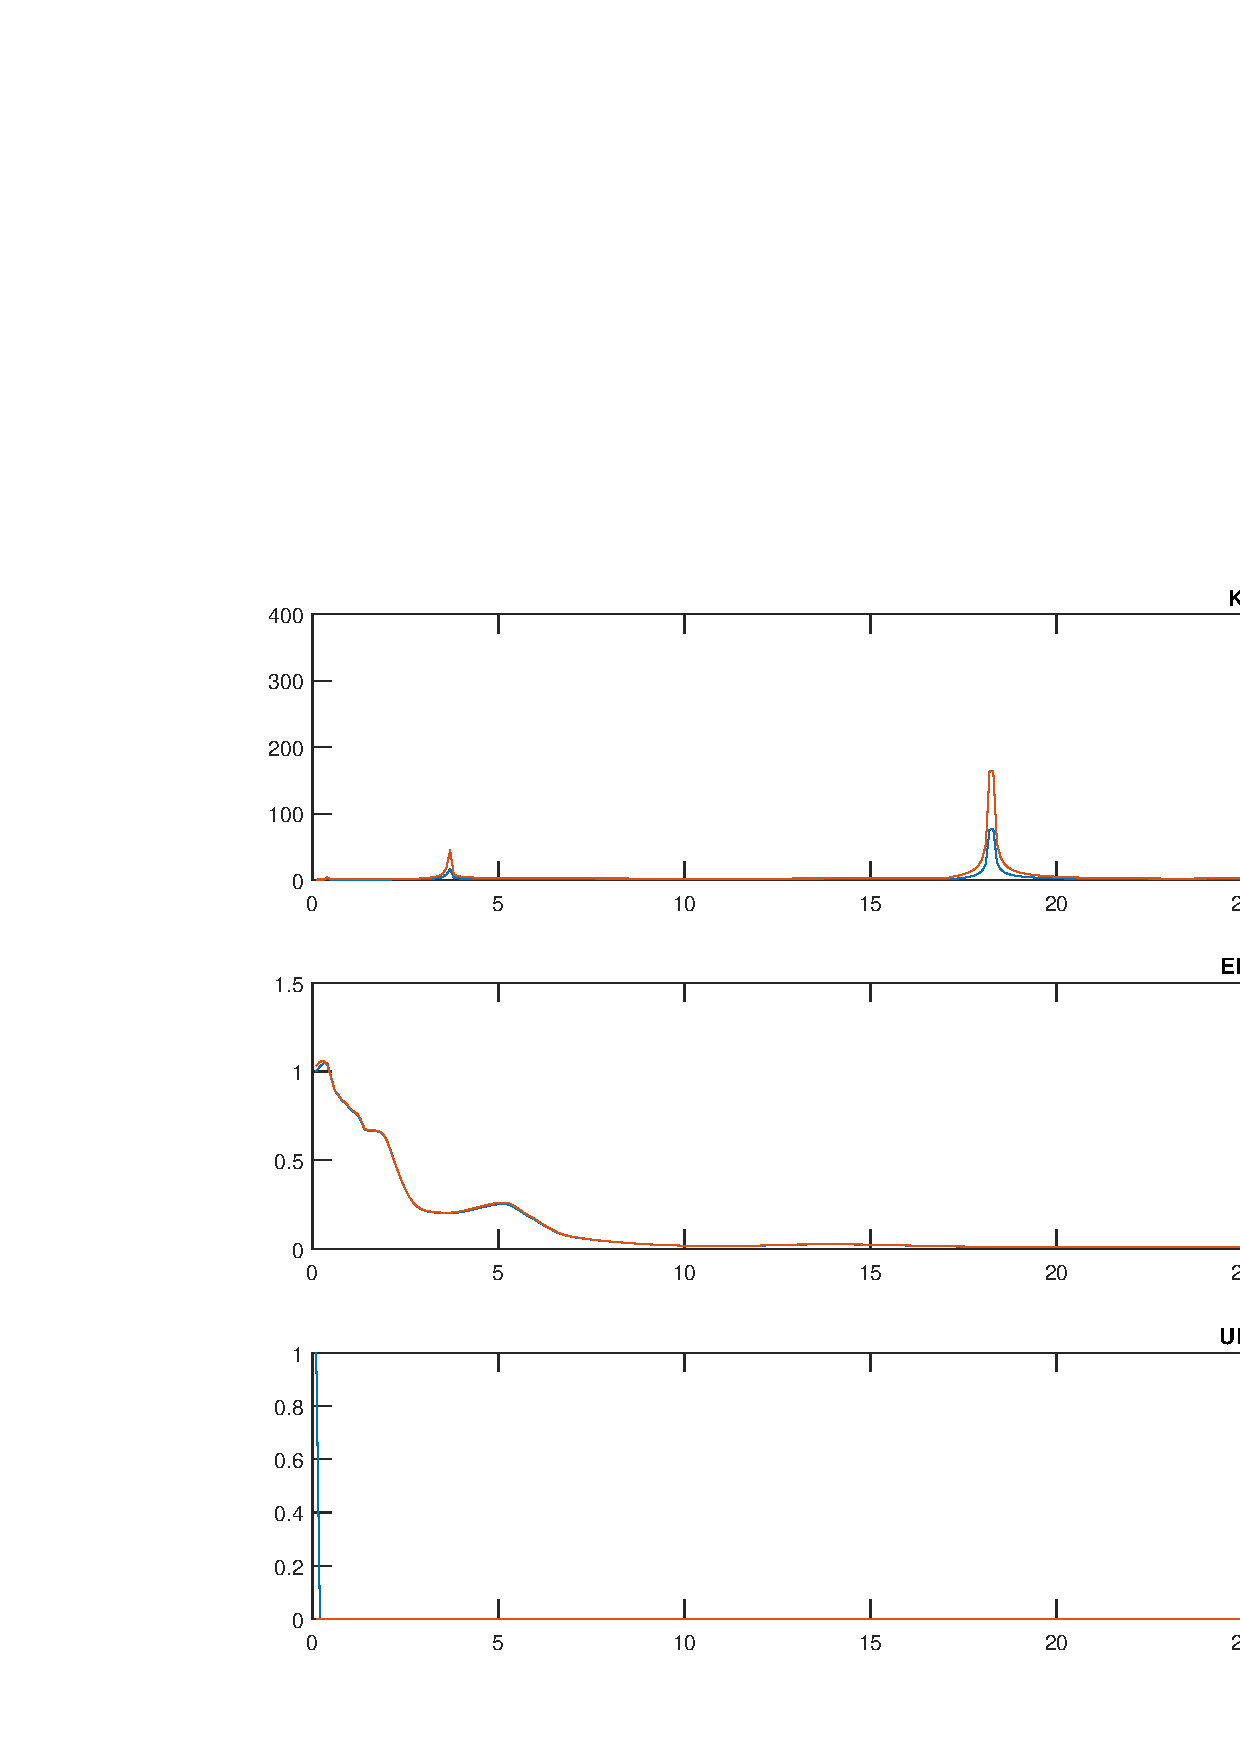
\includegraphics[width=0.8\linewidth]{plots/spectral_radii_all_subplots.png}
\end{figure}
\end{frame}
%------------------------------------------------ESTEIMATION ERROR---------------------
\begin{frame}
\frametitle{Results: Estimation error(All Filter)}

\begin{figure}
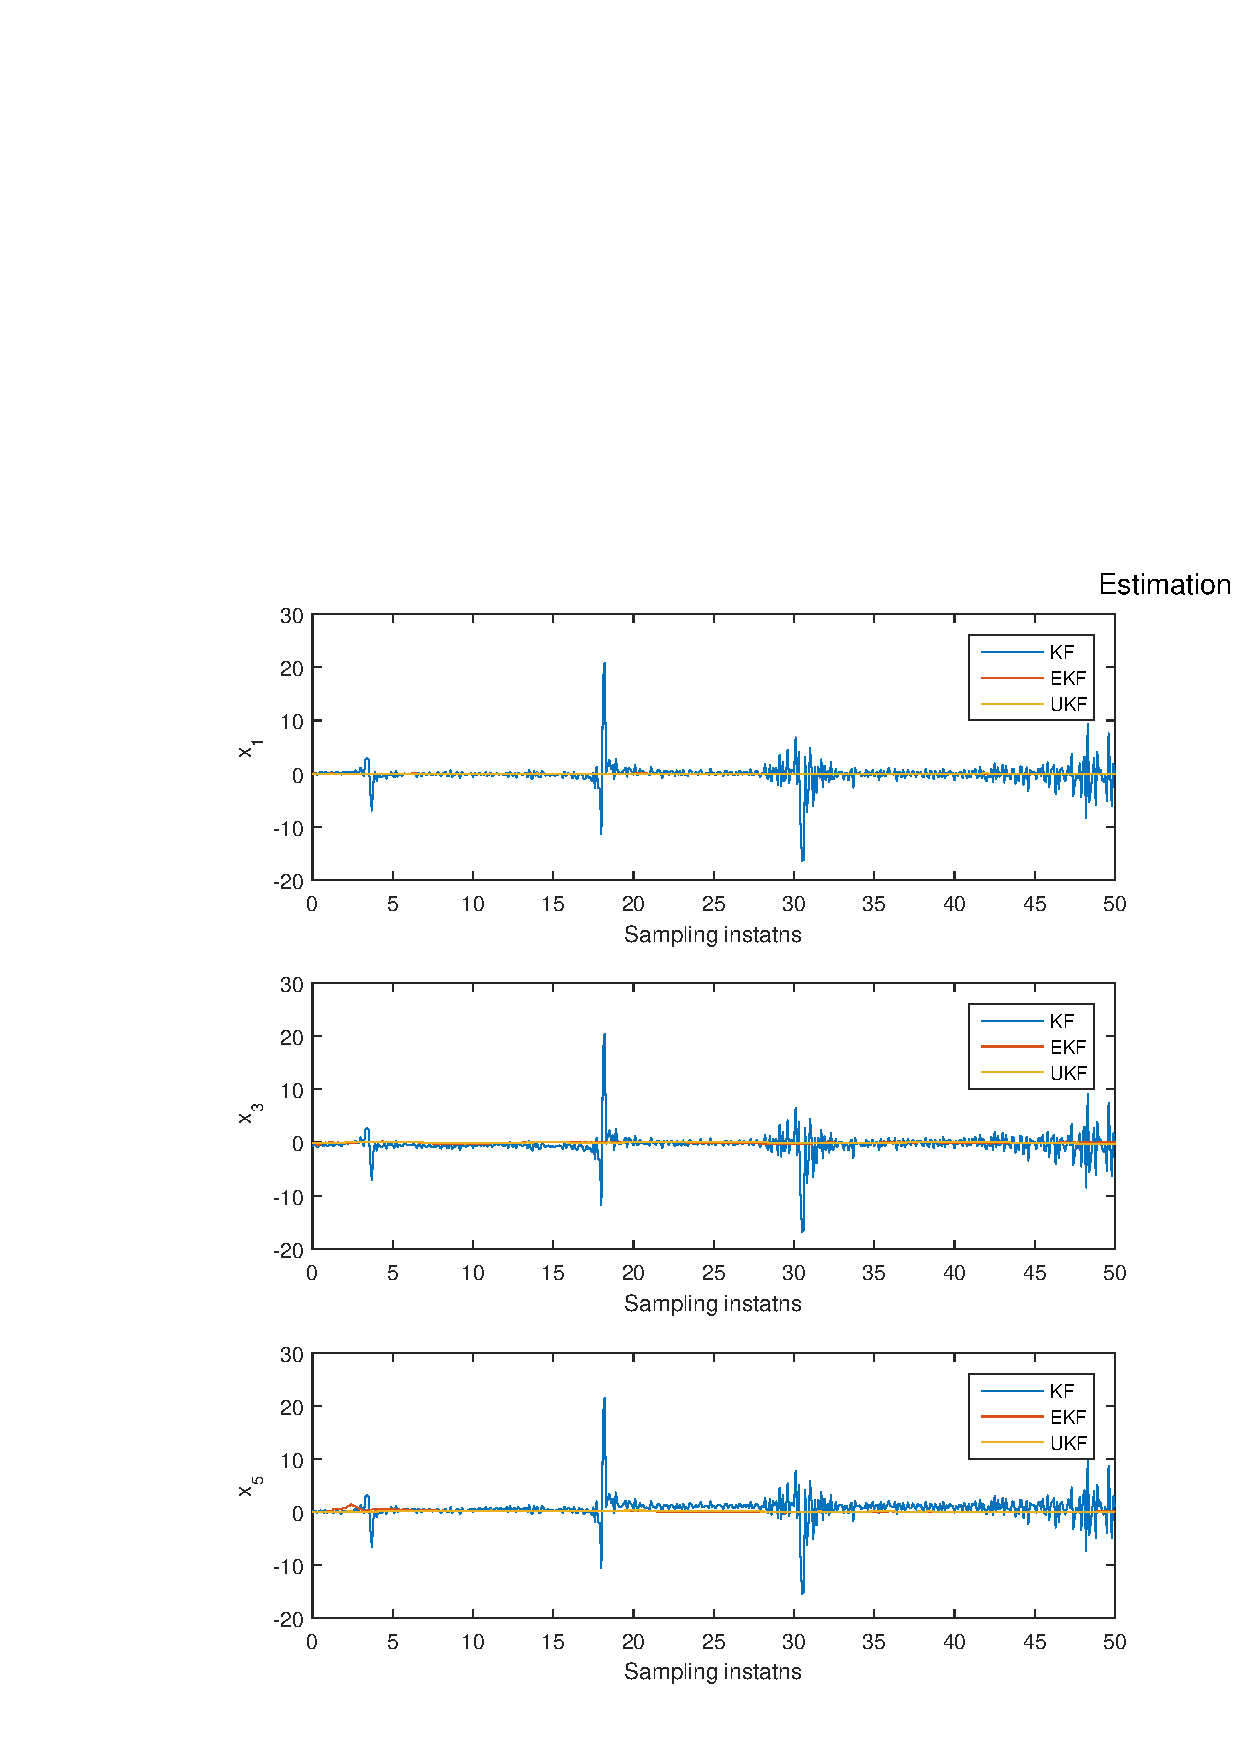
\includegraphics[width=0.8\linewidth]{plots/estimation_error_all.png}
\end{figure}
\end{frame}
%----------------------------------------Estimation Error EKF with std bounds-------
\begin{frame}
\frametitle{Results: Estimation error for EKF}

\begin{figure}
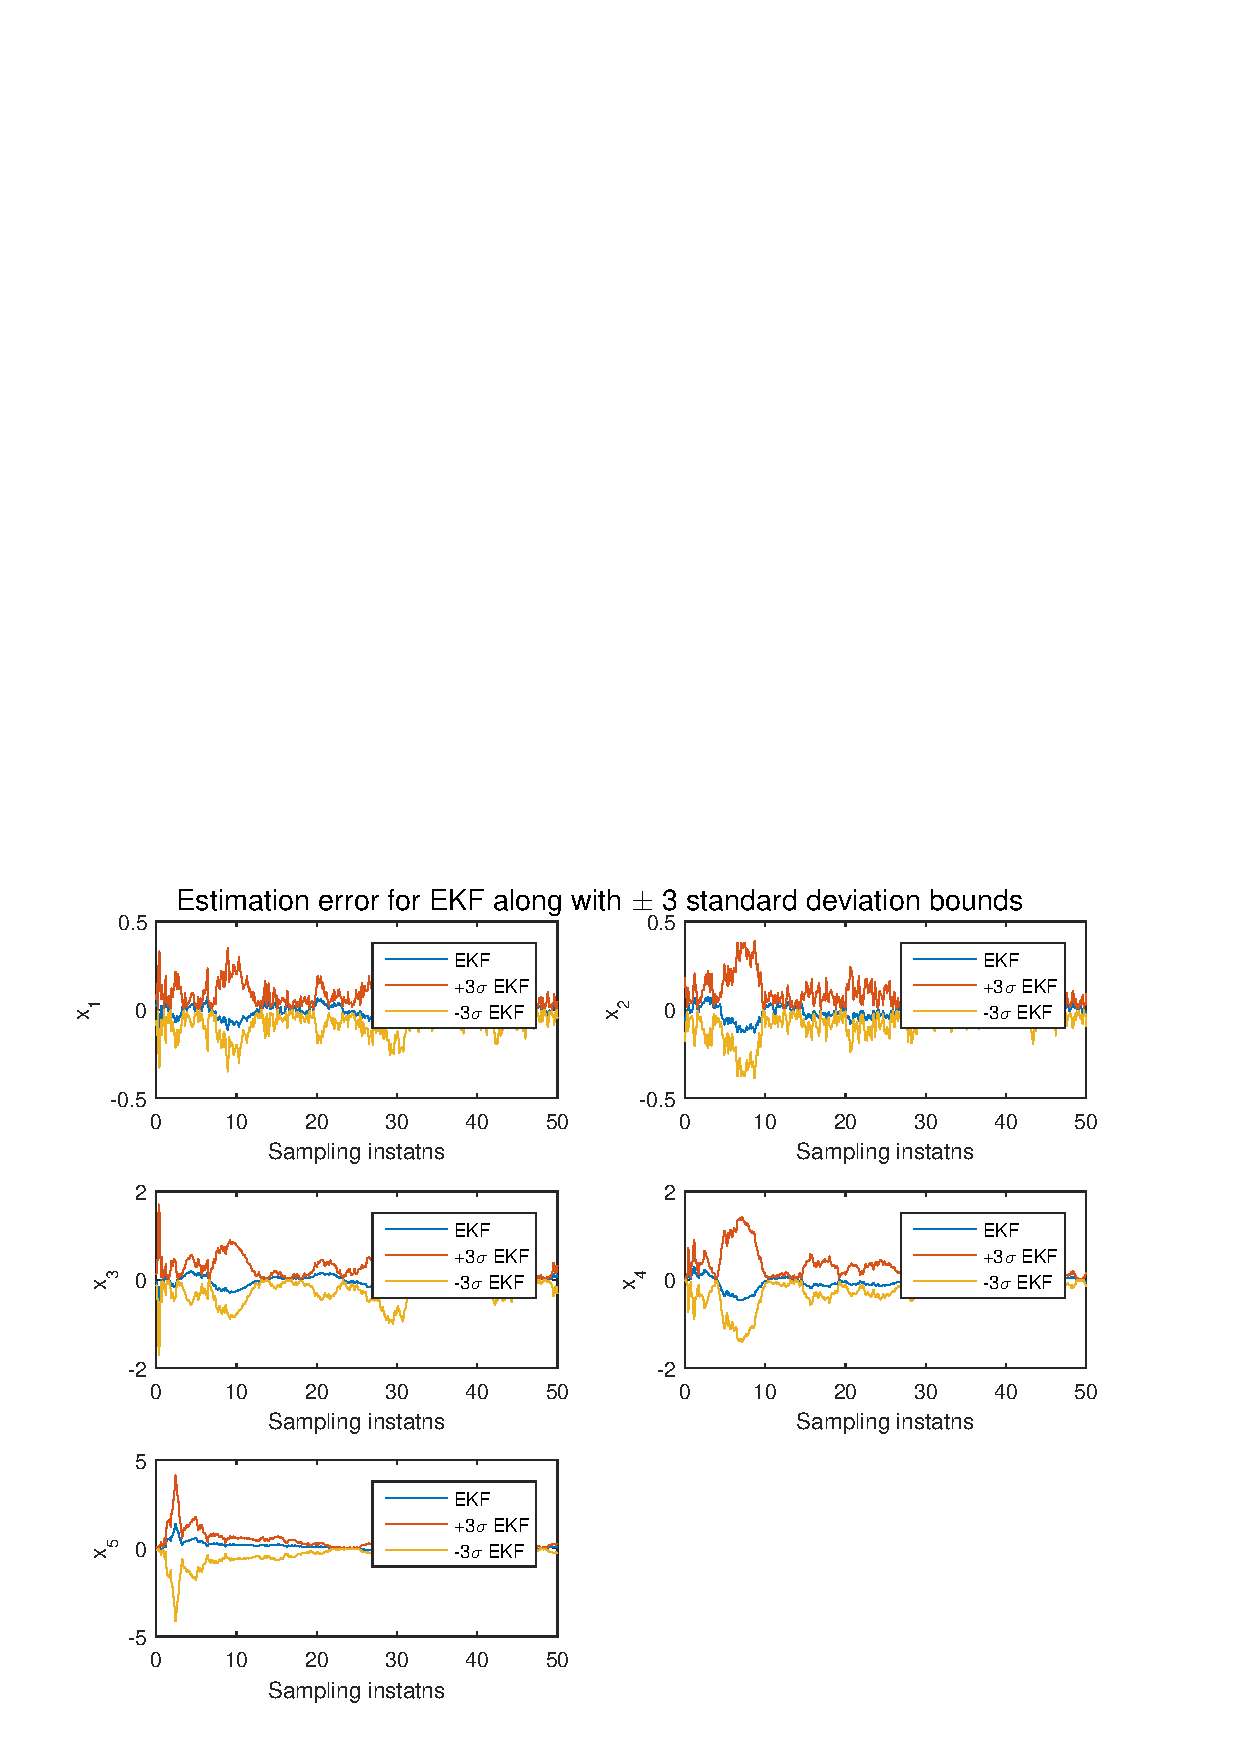
\includegraphics[width=0.8\linewidth]{plots/estimation_error_EKF_sigma_all_states.png}
\end{figure}
\end{frame}
%----------------------------------------Estimation Error UKF with std bounds-------
\begin{frame}
\frametitle{Results: Estimation error for UKF}

\begin{figure}
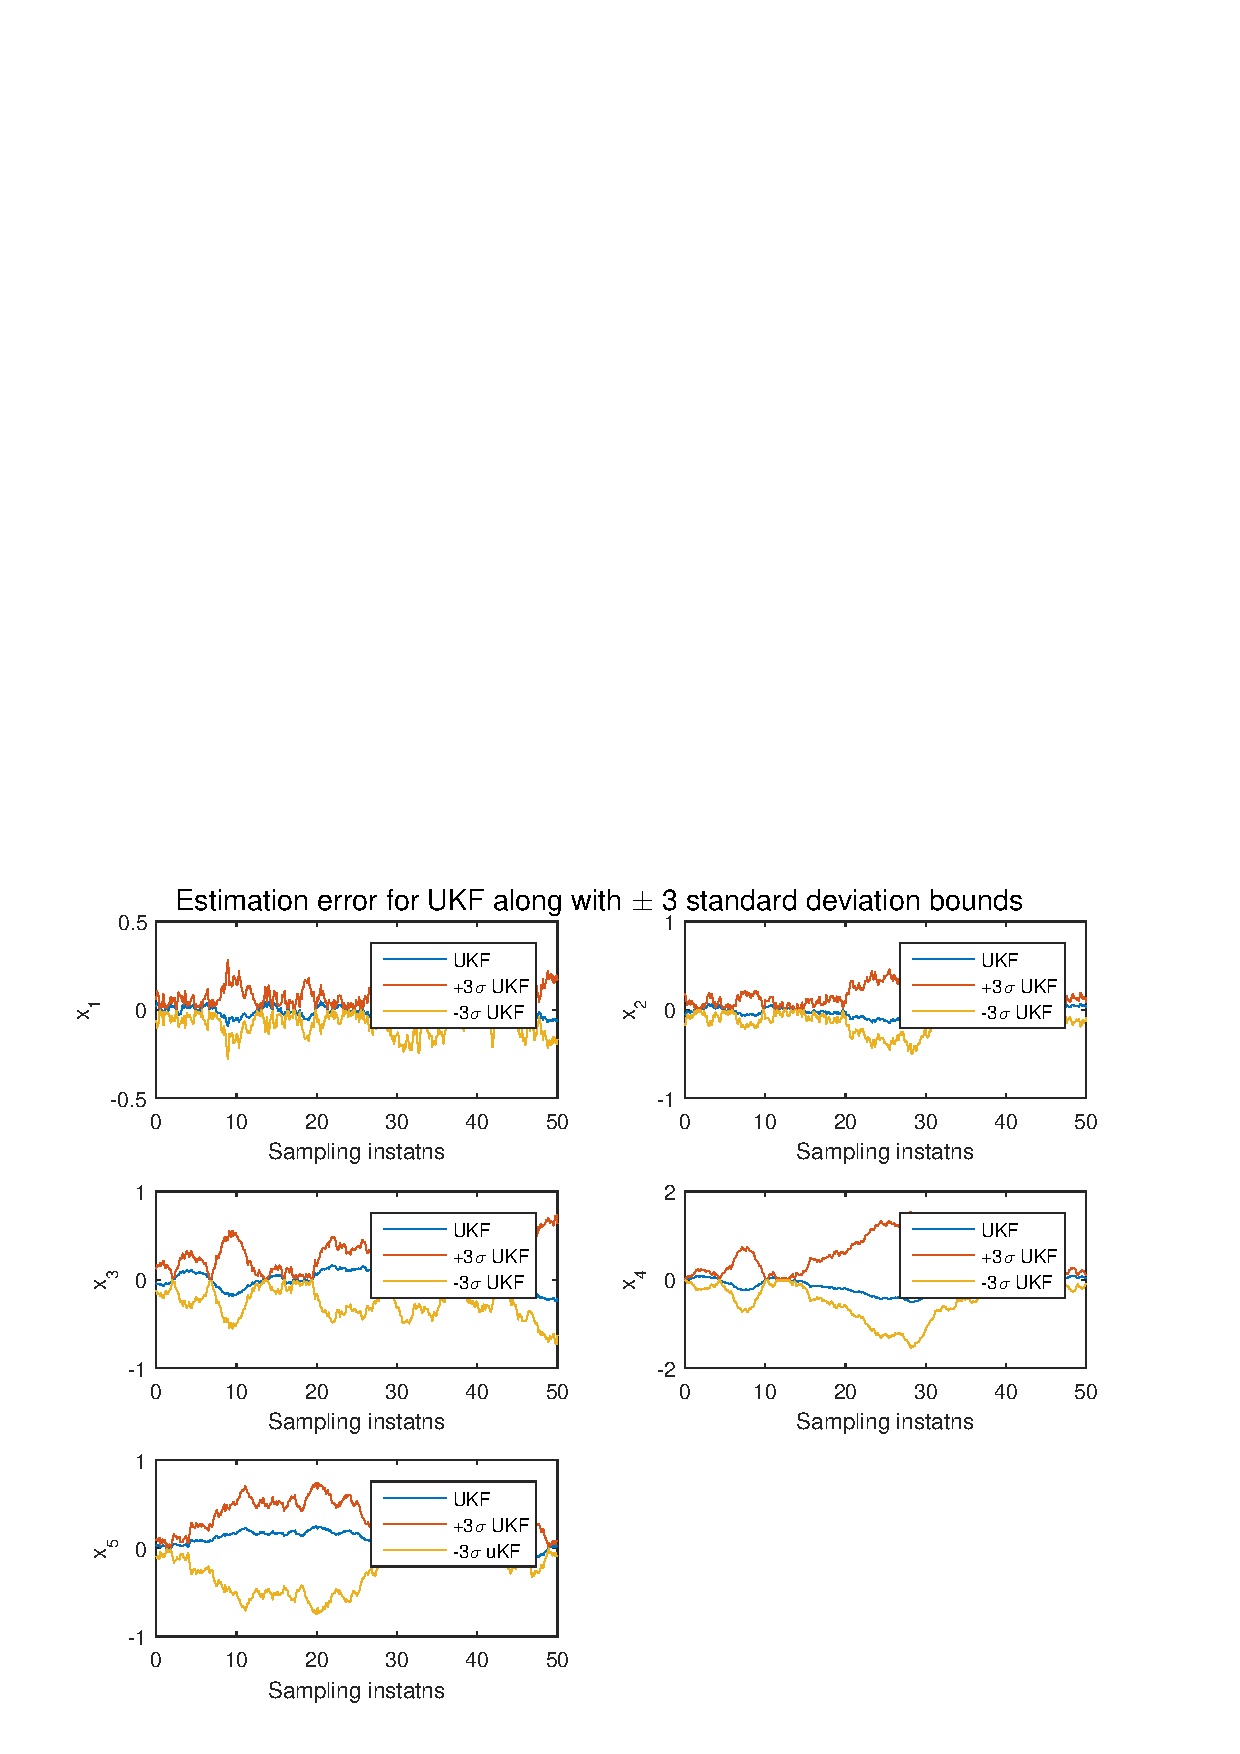
\includegraphics[width=0.8\linewidth]{plots/estimation_error_UKF_sigma_all_states.png}
\end{figure}
\end{frame}
%---------------------Estimation error EKF,UKF with std bounds on same plot-----------------
\begin{frame}
\frametitle{Results: Estimation error for EKF and UKF(State 1)}
\begin{figure}
\includegraphics[width=0.8\linewidth]{plots/estimation_error_noKF_sigma_s1.png}
\end{figure}
\end{frame}
%------------------------------------------------
\begin{frame}
\frametitle{Results: Estimation error for EKF and UKF(State 2)}
\begin{figure}
\includegraphics[width=0.8\linewidth]{plots/estimation_error_noKF_sigma_s2.png}
\end{figure}
\end{frame}
%------------------------------------------------
\begin{frame}
\frametitle{Results: Estimation error for EKF and UKF(State 3)}
\begin{figure}
\includegraphics[width=0.8\linewidth]{plots/estimation_error_noKF_sigma_s3.png}
\end{figure}
\end{frame}
%------------------------------------------------
\begin{frame}
\frametitle{Results: Estimation error for EKF and UKF(State 4)}
\begin{figure}
\includegraphics[width=0.8\linewidth]{plots/estimation_error_noKF_sigma_s4.png}
\end{figure}
\end{frame}
%------------------------------------------------
\begin{frame}
\frametitle{Results: Estimation error for EKF and UKF(State 5)}
\begin{figure}
\includegraphics[width=0.8\linewidth]{plots/estimation_error_noKF_sigma_s5.png}
\end{figure}
\end{frame}
%% ------------TABLES------------------------
% will have to make image of tables
\begin{frame}{Tables}
    \begin{figure}
        \centering
        \includegraphics[width=0.8\linewidth]{plots/tables.PNG}
        \caption{Mean,Variance and RMSE for filters}
        \label{fig:my_label}
    \end{figure}
\end{frame}
%---------------------NESS-----Beta_K plots----------------------
\begin{frame}
\frametitle{Results:Normalised Estimation Error Squared(NESS)}
\begin{figure}
\includegraphics[width=0.8\linewidth]{plots/betak_all.png}
\end{figure}
\end{frame}
%------------------------------------------------
\begin{frame}
\frametitle{Results: Normalised Estimation Error Squared(NESS)}
\begin{figure}
\includegraphics[width=0.8\linewidth]{plots/betak_noKF.png}
\end{figure}
\end{frame}
%------------------------------------------------
\section{Conclusion}
\begin{frame}{Conclusion}
    \begin{itemize}
        \item The fraction of time instants for which $\beta_k$ exceeded the bounds was 0 and $\alpha$=0.05. Hence filter can be said consistent.
        \item KF didn't work well on this system at chose linearisation point.
        \item Both EKF and UKF performed decently well.
        \item For few states EKF estimated better, for few UKF and for few both did better
    \end{itemize}
\end{frame}
%------------------------------------------------
\section{References}
\begin{frame}
\frametitle{References}
\begin{itemize}
    \item Lectrue slides
    \item Kandepu, R., and Foss, B., and Imsland, L.; Applying the Unscented Kalman Filter
for Nonlinear State Estimation, Journal of Process Control, 18, 2008, 753-768.
\end{itemize}
\end{frame}

%------------------------------------------------

\begin{frame}
\Huge{\centerline{The End}}
\end{frame}
%----------------------------------------------------------------------------------------

\end{document}